% =====================================================================
% ICISSP 2027 -- Paper #21 -- CIGMA
% LaTeX source RECONSTRUCTED on 21/11/2026 from the submitted PDF
% (ICISSP_2027_21_1.pdf, initial anonymous version, 8 pages).
% Text, equations, tables and references transcribed from the PDF.
% Figures 1-3 are the raster images extracted from the PDF
% (the original vector/plot sources were not available).
% Chantier 122-CIGMA-ICISSP (suivi Overleaf yulliwas-ameur).
% =====================================================================
\documentclass[a4paper,twoside]{article}

\usepackage[utf8]{inputenc}
\usepackage[T1]{fontenc}
\usepackage[english]{babel}
\usepackage{graphicx}
\usepackage{amsmath,amssymb}
\usepackage{booktabs,array}
\usepackage{balance}
\usepackage{algorithm2e}
% indicator function (original PDF used a double-struck 1; \mathbbm{1} from bbm works on Overleaf)
\usepackage{xspace}
\usepackage{url}
\usepackage[hidelinks]{hyperref}
% Double-blind: scrub PDF metadata.
\hypersetup{pdfauthor={},pdftitle={},pdfsubject={},pdfkeywords={}}
\usepackage{pslatex}
\usepackage{apalike}
\usepackage{SCITEPRESS}
\addto\captionsenglish{\renewcommand{\refname}{REFERENCES}}

% ---------------------------------------------------------------------
% Macros
% ---------------------------------------------------------------------
\newcommand{\cigma}{CIGMA\xspace}
\newcommand{\rel}[1]{\textsc{#1}}          % relation names (small caps)
\newcommand{\meth}[1]{\textsf{#1}}         % method / baseline names
\newcommand{\verify}{\textsc{Verify}\xspace}

\begin{document}

\title{CIGMA: Provenance-Preserving Cryptographic Dependency\\Reconstruction for Post-Quantum Network Migration}

\author{\authorname{Anonymous Author(s)}
\affiliation{Author names and affiliations omitted for double-blind review}}

\keywords{Post-Quantum Cryptography, Cryptographic Inventory, Network Dependency Graph, Crypto-Agility, Provenance, Entity Resolution, Network Security.}

\abstract{Post-quantum migration is a network dependency problem before it is an algorithm-replacement problem: operators must connect certificates, protocols, libraries, deployment pipelines, services, and devices before sequencing changes without breaking communicating peers. We present \cigma, a deterministic pipeline that fuses heterogeneous cryptographic observations into a typed dependency graph while retaining locator-backed provenance for every accepted node and edge. A closed ontology, quality gate, stable identity rules, and allow-listed path composition form an executable contract; impact, migration feasibility, and evidence support remain separate. We evaluate \cigma on CIGMA-Lab, an oracle-separated, six-source reference infrastructure with 46 entity and 34 relation observations. On the complete fixture, \cigma attains asset, pairwise entity-resolution, B$^3$, and typed-edge F1 of 1.0000, versus typed-edge F1 0.8529 for an observation union and 0.8923 for exact-ID and TF--IDF comparators. Across 384 paired runs under seeded observation deletion, the asset advantage over exact matching remains material, whereas the relational advantage becomes negligible at 50\% deletion, exposing a clear evidence-availability boundary. A separately sealed 30-call optional-model study shows fail-closed validation raising candidate F1 from 0.9361 to 0.9554 without admitting an oracle-false triple. The study establishes reproducible network-dependency reconstruction on one controlled system; independent deployed-system validation remains necessary.}

\onecolumn \maketitle \normalsize \setcounter{footnote}{0} \vfill

% =====================================================================
\section{\uppercase{Introduction}}
\label{sec:intro}
% =====================================================================

NIST standardized ML-KEM, ML-DSA, and SLH-DSA in 2024 \cite{nist2024fips203,nist2024fips204,nist2024fips205}. The resulting transition is often described as replacing vulnerable public-key algorithms, but enterprise deployment makes it a distributed-systems problem. A TLS endpoint can be observed by a network scanner, its certificate by a PKI export, its implementation by a cryptography bill of materials (CBOM), its deployment by CI/CD metadata, and its business lifetime by a service catalog. None of these views alone identifies the communicating service pair, trust path, deployment owner, or downstream blast radius that determines whether a migration step is safe.

The operational risk has two sides. Incomplete discovery leaves long-lived confidentiality exposure untreated. Incorrect fusion can be equally harmful: duplicate assets distort priorities, false relations create fictitious migration blockers, and missing dependencies can cause interoperability failures when one side of a network relation migrates before the other. Recent PQC guidance therefore emphasizes inventory and crypto-agility \cite{moody2024transition,cisa2024strategy}, while current research increasingly models dependencies and migration order \cite{hasan2024framework,sharma2026dependency,herzinger2026twin}. Yet three gaps remain. First, cryptographic discovery tools usually expose one layer; CBOM tools can disagree substantially \cite{bogli2026bfcbom}. Second, graph-based migration studies often assume that nodes and dependencies are already correct. Third, evidence lineage is rarely evaluated assertion by assertion, even though an operator must be able to audit why a service was linked to a vulnerable primitive.

We address these gaps with \cigma, a provenance-preserving, multi-source cryptographic dependency reconstruction pipeline. Its principal graph is deterministic. Every accepted assertion retains source observation identifiers, locators, excerpts, and hashes; entity resolution uses strong identifiers before constrained aliases; relation signatures and path compositions are closed; and low evidence support triggers verification rather than lowering intrinsic urgency. An optional language model may propose relation candidates, but it cannot create assets or mutate the graph and is evaluated separately.

We ask three questions:
\begin{itemize}
\item \textbf{RQ1 -- Reconstruction:} What do multi-source identity resolution and typed path composition add over single-source inventories, an observation union, exact identifiers, and record similarity?
\item \textbf{RQ2 -- Robustness:} How do asset, relation, provenance, and ranking quality degrade when source families or observations are missing?
\item \textbf{RQ3 -- Bounded model assistance:} Can deterministic validation contain unsupported model-generated relations and add useful evidence-backed edges without changing the principal graph?
\end{itemize}

The contributions are: (i)~a closed, typed network-dependency graph with mandatory locator-backed provenance; (ii)~a deterministic fusion and migration-ordering pipeline that separates urgency, feasibility, and evidence; (iii)~an oracle-isolated benchmark with executable baselines, ablations, source removal, paired dropout, and scaling; and (iv)~a sealed, replayable candidate-only model experiment. The scientific claim is deliberately centered on reconstructing \emph{network cryptographic dependencies}; migration-order effectiveness on a deployed second system remains an external-validation question.

% =====================================================================
\section{\uppercase{Related Work and Research Gap}}
\label{sec:related}
% =====================================================================

\subsection{PQC Migration and Dependency Planning}

Hasan \emph{et al.} combine organizational inventories with graph-theoretic dependency analysis \cite{hasan2024framework}; a systematic review finds real software migrations heterogeneous and largely experimental \cite{nather2024migrating}. CARAF frames lack of agility as operational risk \cite{ma2021caraf}. More recent work derives migration order from dependency graphs: Sharma \emph{et al.} report faster cumulative risk reduction and fewer interoperability failures under dependency-aware ordering \cite{sharma2026dependency}, while infrastructure twins and architecture-derived CBOMs add system context \cite{herzinger2026twin,hess2026anatomy}. These approaches motivate network-aware migration but generally take the inventory graph as input. \cigma instead evaluates how that graph is reconstructed from conflicting partial observations.

\subsection{Cryptographic Discovery, CBOMs, and Graph Fusion}

Inventory requirements span software, hardware, communications, stored data, and source code \cite{schmitt2024criteria}. Static tools can detect defined cryptographic assets and misuse classes \cite{rahaman2019cryptoguard}; recent work evaluates discovery on a synthetic benchmark and a deployed ten-service infrastructure \cite{nather2026hidden}. CBOM orchestration studies expose major inter-tool discrepancies \cite{bogli2026bfcbom}. Security knowledge graphs integrate heterogeneous sources \cite{sikos2023cybersecurity}, and provenance-aware graphs retain source lineage \cite{mitra2021provenance}. However, scale or query demonstrations do not by themselves establish entity and typed-edge correctness.

\subsection{Entity-Resolution Evaluation}

Entity resolution must be evaluated both pairwise and as clustering. Entity-centric benchmark construction supports pairwise and cluster metrics together with root-cause error analysis \cite{binette2024entity,binette2023ereval}. Multi-source settings also require robustness to source order and source composition \cite{saeedi2020incremental}. \cigma therefore reports asset, pairwise, B$^3$, and typed-edge measures; separates duplicate, unmappable, and oracle-absent edge errors; and evaluates fixed paired deletion masks.

Table~\ref{tab:positioning} shows the resulting distinction. The novelty is not ``a graph for PQC'' in isolation; it is the measured composition of multi-source resolution, typed dependency reconstruction, and mandatory evidence lineage.

\begin{table*}[t]
\caption{Positioning of representative approaches. ``Measured graph'' means labeled entity or typed-edge evaluation, not only a case study or query demonstration.}
\label{tab:positioning}
\centering
\small
\setlength{\tabcolsep}{4pt}
\begin{tabular}{@{}lccccc@{}}
\toprule
Approach & Multi-src. & Typed & Lineage & PQC & Measured \\
\midrule
Static crypto scan \cite{rahaman2019cryptoguard,nather2026hidden} & -- & partial & file/line & partial & asset \\
CycloneDX/CBOM \cite{hess2026anatomy,bogli2026bfcbom} & partial & partial & partial & partial & partial \\
Security KG \cite{sikos2023cybersecurity,mitra2021provenance} & yes & yes & varies & -- & varies \\
PQC planning \cite{hasan2024framework,sharma2026dependency} & partial & yes & partial & yes & partial \\
\cigma & yes & yes & mandatory & yes & entity+edge \\
\bottomrule
\end{tabular}
\end{table*}

% =====================================================================
\section{\uppercase{CIGMA Design}}
\label{sec:design}
% =====================================================================

\subsection{Observation and Graph Model}

A source family $s$ emits entity and relation observations. An entity observation is
\begin{equation}
o = \langle id, s, k, T, I, A, q, \tau, \ell, e, H(e) \rangle ,
\label{eq:observation}
\end{equation}
where $k$ is a source-local key, $T$ a declared type, $I$ identifiers, $A$ attributes, $q \in [0,1]$ configured observation quality, $\tau$ collection time, $\ell$ a locator, $e$ a retained excerpt, and $H(e)$ its SHA-256 digest. Relation observations add subject, predicate, and object observations. The digest protects the retained excerpt; it is not presented as authentication of an unarchived upstream system.

\begin{figure}[t]
\centering
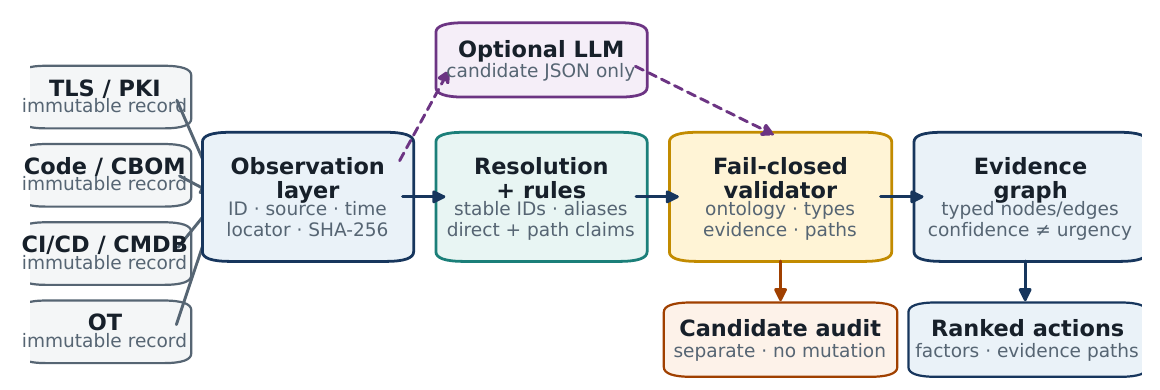
\includegraphics[width=\columnwidth]{figures/fig1-dataflow.png}
\caption{Deterministic \cigma data flow. The optional model proposes candidate JSON only; validation and audit remain separate from the principal graph.}
\label{fig:dataflow}
\end{figure}

The graph $G = (V, E, \phi_V, \phi_E, \Pi)$ contains eight entity types: service, endpoint, certificate, algorithm, software component, pipeline, data class, and device. Relations are \rel{hosts}, \rel{presents}, \rel{uses}, \rel{issued-by}, \rel{depends-on}, \rel{deploys}, \rel{processes}, and \rel{protects}, each with explicit domain and range. $\Pi(a)$ returns the evidence observations supporting assertion $a$. Construction fails closed if an accepted node or edge has no valid provenance.

\subsection{Stable Identity Resolution}

Strong keys include certificate or SPKI fingerprint, PURL, service UID, device serial, algorithm ID, endpoint URI, pipeline UID, and data UID. Service name, hostname, repository path, and deployment name are weaker aliases. Alias merging is allowed only for type-compatible clusters with no conflicting strong identifier. Canonical IDs hash the entity type and a deterministic identifier anchor, making output independent of ingestion order and model wording. The resolution log records every match rule and value.

Observations below the quality gate are quarantined. Numeric values are aggregated by quality--source-reliability weighted mean, Boolean values by weighted majority, and categorical values by support. Direct relations are type checked and grouped by canonical triple. Derived \rel{service uses algorithm} edges are limited to two declared forms: \rel{hosts}$\circ$\rel{presents}$\circ$\rel{uses} and \rel{uses}$\circ$\rel{uses}. Each derived edge carries the union of path evidence. Figure~\ref{fig:dataflow} summarizes these boundaries.

\subsection{Evidence and Migration Order}

For observation $i$ with quality $q_i$ and source reliability $r_i$, $p_i = q_i r_i$. Node support is $c_v = 1 - \prod_i (1 - p_i)$. A direct relation observation $j$ receives support $d_j = q_j r_j \sqrt{c_s c_o}$, clipped to $[0,1]$; repeated observations combine by noisy-OR. A length-$k$ path uses $\min_h c_{e_h} \lambda^{k-1}$. These are auditable support scores, not externally calibrated probabilities.

The impact vector is $\mathbf{r}_v = (Q, H, C, X, B)$: quantum vulnerability, HNDL urgency, criticality, exposure, and normalized transitive service dependents. With confidentiality lifetime $L$, migration time $M$, policy horizon $z$, and service set $V_S$,
\begin{equation}
H = Q \min\!\left(1, \frac{L+M}{z}\right),;
B = \max_{s \in S(v)} \frac{|D(s)|}{\max(1, |V_S| - 1)} .
\label{eq:impact}
\end{equation}
Unknown factors produce lower/upper decision vectors by substituting 0/1. The primary order uses descending upper and lower policy tiers, Pareto fronts within an equal tier interval, then a deterministic lexicographic tie-break. Evidence support cannot lower urgency; a potentially high-impact item with uncertain factors or low support enters \verify. A weighted sum remains only a comparator.

\subsection{Optional Bounded Model}

The principal graph uses no model. When explicitly enabled, the adapter receives existing graph IDs and types, public observations, the closed predicate vocabulary, and allowed paths. It cannot create canonical nodes, access the oracle, receive computed rankings, invoke tools, or write to the graph. Strict structured output constrains shape; deterministic validation checks node existence, type signatures, evidence membership in accepted direct edges, and exact direct or allow-listed path support. Accepted and rejected candidates are archived separately with \texttt{graph\_mutated=false}.

\subsection{End-to-End Dependency Trace}

A concrete trace illustrates the difference between an inventory item and a network migration dependency. First, a TLS record at locator \texttt{sslyze/edge.json\#} \texttt{/certificate\_deployments/0} states that endpoint \texttt{tls://edge.local:443} presents certificate fingerprint \texttt{FPR-EDGE-RSA-001}. Normalization creates endpoint, certificate, and \rel{presents} observations while preserving their IDs and locator. Second, an independent PKI export reports the same fingerprint, its RSA key, and issuer; fingerprint equality merges the certificate observations but preserves both evidence records. Third, a CMDB observation links the edge service to the same endpoint URI through \rel{hosts}. Once the direct edges pass the quality and ontology gates, the declared path \rel{hosts}$\circ$\rel{presents}$\circ$\rel{uses} derives that the service uses RSA-2048 and carries the union of TLS and PKI evidence. If any accepted path edge is absent, the service-level relation is absent rather than guessed.

For the resulting service, $Q=1$, confidentiality lifetime $L = 2$ years, migration time $M = 1.5$ years, and $z = 10$ give $H = 0.35$. With criticality 0.80, exposure 1, and blast radius 0, the item lies in tier interval $[2,2]$, Pareto front 1. Evidence support 0.771 is below the 0.85 verification threshold, so the item remains urgent and enters \verify. This trace binds a migration decision to auditable network and PKI evidence rather than to an unexplained score.

% =====================================================================
\section{\uppercase{Evaluation Methodology}}
\label{sec:method}
% =====================================================================

\subsection{Reference Infrastructure and Oracle Isolation}

CIGMA-Lab is a structured generated infrastructure, not a production cyber range. Figure~\ref{fig:topology} contains a web/PKI zone, DevOps zone, and OT zone. Six source families expose complementary evidence (Table~\ref{tab:sources}). The public tree contains no oracle identifiers. An evaluator-only tree stores 23 canonical entities, 34 typed edges, observation-to-truth maps, 16 critical migration targets, and author-defined priorities.

The fixture has 46 entity observations: 44 map to oracle entities and two are distractors. Its 34 relation observations include 32 true and two false claims; the true observations collapse to 29 unique direct triples, while five oracle relations require allow-listed composition. Equality between 34 public claims and 34 oracle edges is therefore coincidental.

\begin{figure}[t]
\centering
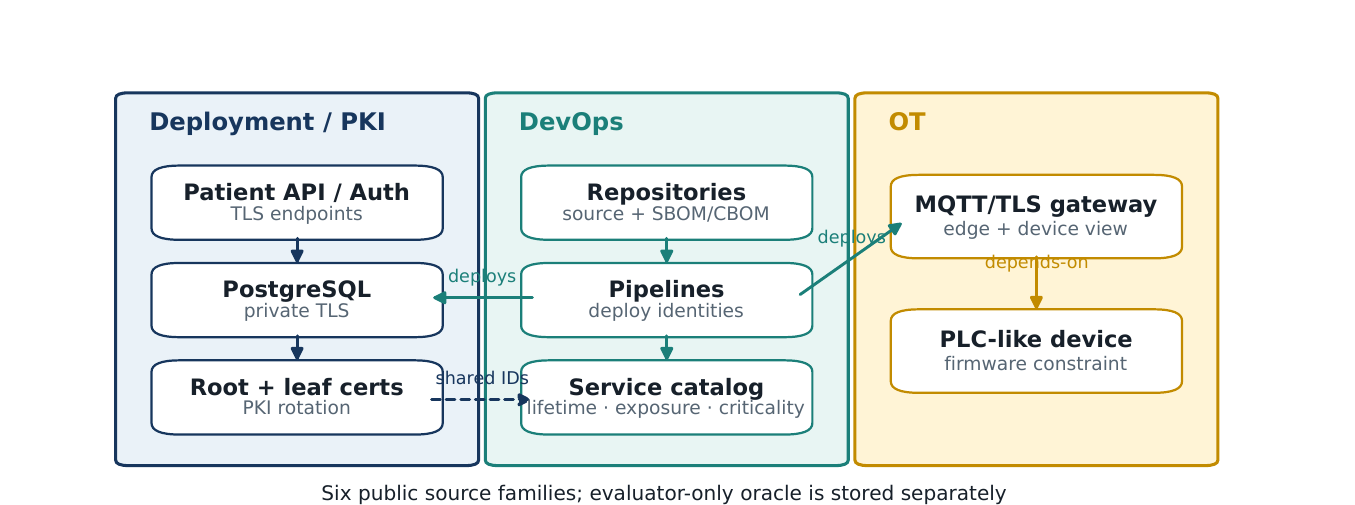
\includegraphics[width=\columnwidth]{figures/fig2-cigma-lab-topology.png}
\caption{CIGMA-Lab network and deployment topology. The same asset appears through multiple modalities, forcing cross-source resolution.}
\label{fig:topology}
\end{figure}

\begin{table}[t]
\caption{Directly observable content by source family.}
\label{tab:sources}
\centering
\small
\begin{tabular}{@{}l>{\raggedright\arraybackslash}p{3.6cm}>{\raggedright\arraybackslash}p{1.5cm}@{}}
\toprule
Source & Direct evidence & Identifier \\
\midrule
TLS & endpoint, protocol, presented leaf, algorithm & URI, fingerprint \\
PKI & certificate, issuer, key, rotation & fingerprint \\
CBOM & service alias, package, crypto use & PURL, path \\
CI/CD & pipeline, deployed service & stable UID \\
CMDB & service, lifetime, exposure, data & service/data UID \\
OT & gateway/device dependency, crypto & serial number \\
\bottomrule
\end{tabular}
\end{table}

\subsection{Methods, Ablations, and Perturbations}

We compare: \meth{TLSInventory}; \meth{CBOMInventory}; \meth{SourceUnion}, retaining one node per observation; \meth{ExactDirect}, using strong identifiers and direct claims; \meth{TFIDF-Cosine}, using scikit-learn character TF--IDF and cosine similarity at a fixed 0.80 threshold without oracle tuning \cite{pedregosa2011scikit}; and full \cigma. Ablations remove aliases, paths, the quality gate, or source-reliability differences.

Robustness uses six leave-one-source-out conditions and deletion probabilities 0, 0.10, 0.25, and 0.50. At each level, 32 seed-indexed paired masks are applied to \meth{SourceUnion}, \meth{ExactDirect}, and \cigma, yielding 384 method runs. Claims are eligible only if endpoints survive, so relations disappear faster than entities. All parameters are frozen before evaluation.

\subsection{Metrics and Statistics}

Asset F1 gives one true positive per distinct oracle entity; duplicate and unmapped clusters are false positives. Resolution additionally uses pairwise and B$^3$ scores \cite{binette2023ereval}. Typed-edge metrics compare canonical triples and partition false positives into duplicate oracle-true edges, unmappable endpoints, and mapped oracle-absent triples. Evidence-unsupported rate is separate. Ranking uses operational NDCG@5/10 \cite{jarvelin2002cumulated} and Kendall $\tau_b$, where duplicate clusters occupy zero-relevance positions. We also report critical misses, verification-queue size, Brier/ECE diagnostics \cite{guo2017calibration}, and runtime.

For each metric and dropout level, percentile 95\% bootstrap intervals use 5,000 resamples \cite{efron1979bootstrap}. \cigma-minus-baseline differences use paired bootstrap and two-sided sign randomization; Holm correction covers 24 planned contrasts \cite{holm1979simple}. The unit is a deletion mask, not a node or edge. The 30-call model cohort uses call-level bootstrap and six predeclared paired contrasts; its intervals quantify one request and service window, not independent systems.

% =====================================================================
\section{\uppercase{Results}}
\label{sec:results}
% =====================================================================

\subsection{Reconstruction and Ablation (RQ1)}

Table~\ref{tab:reconstruction} reports complete-fixture reconstruction. Single-source inventories each miss ten of 16 critical targets. \meth{SourceUnion} preserves all observations but cannot resolve duplicates, giving pairwise entity F1 0.0000 and asset F1 0.6667. \meth{ExactDirect} and \meth{TFIDF-Cosine} improve identity quality but miss aliases and allowed cross-layer paths. \cigma reconstructs all 23 entities and 34 edges: all four F1 measures equal 1.0000, edge-FP and evidence-unsupported rates are 0, and no critical target is missed.

Ablations identify the mechanisms. Removing aliases lowers asset F1 to 0.9200 and introduces edge errors; removing path composition leaves assets intact but lowers edge F1 to 0.9206; removing the quality gate lowers asset F1 to 0.9583 and raises edge FP to 0.0556. Setting all source reliabilities to one leaves reconstruction unchanged but reduces the verification queue from 15 to seven, confirming that support assumptions affect verification rather than truth reconstruction.

The primary order reaches NDCG@5/10 0.8948/0.8984 and $\tau_b = 0.2737$. A naive weighted comparator is slightly higher (0.9106/0.9129 and 0.3648). We therefore do not claim empirical ranking superiority. The weight-free policy is retained for non-compensation and auditability; expert-adjudicated migration preferences are still required.

\begin{table*}[t]
\caption{Complete-fixture reconstruction. ``Entity'' is pairwise ER F1; Edge FP is the fraction of duplicate, unmappable, or oracle-absent predicted edges.}
\label{tab:reconstruction}
\centering
\small
\begin{tabular}{@{}lrrrrrr@{}}
\toprule
Method & Asset & Entity & B$^3$ & Edge & FP & Miss \\
\midrule
TLS-only & .5161 & .0526 & .1259 & .3000 & .0000 & 10 \\
CBOM-only & .5455 & .0000 & .1549 & .2927 & .1429 & 10 \\
SourceUnion & .6667 & .0000 & .6866 & .8529 & .1471 & 0 \\
ExactDirect & .8846 & .8788 & .9419 & .8923 & .0645 & 0 \\
TFIDF-Cosine & .8519 & .8438 & .9268 & .8923 & .0645 & 0 \\
\cigma & \textbf{1.0000} & \textbf{1.0000} & \textbf{1.0000} & \textbf{1.0000} & \textbf{.0000} & \textbf{0} \\
\bottomrule
\end{tabular}
\end{table*}

\begin{figure*}[t]
\centering
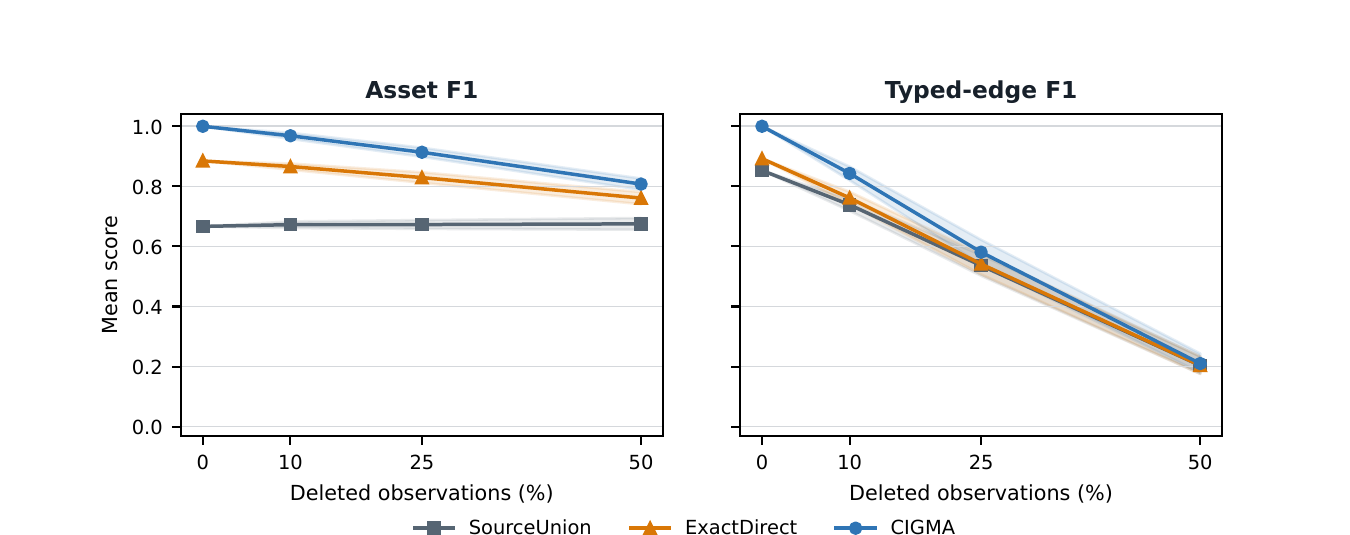
\includegraphics[width=0.78\textwidth]{figures/fig3-deletion-f1.png}
\caption{Mean asset and typed-edge F1 under paired observation deletion. Shading is the percentile 95\% bootstrap interval over 32 masks.}
\label{fig:deletion}
\end{figure*}

\subsection{Missing Evidence and Source Robustness (RQ2)}

Figure~\ref{fig:deletion} shows paired deletion results. At 10\% nominal entity deletion, realized claim deletion is 25.9\%; \cigma retains asset F1 0.9684 and edge F1 0.8430. At 25\%, asset/edge F1 is 0.9135/0.5809. At 50\%, it is 0.8075/0.2101, NDCG@10 is 0.8148, and critical-miss rate is 0.3262. Relations decay faster because every path component must survive.

At 50\%, paired \cigma--\meth{ExactDirect} differences are +0.0465 for asset F1, +0.0061 for edge F1, and +0.0992 for NDCG@5 after multiplicity correction. The edge median is 0 with 9 wins and 23 ties: the relational gain is statistically detectable but practically negligible under severe evidence loss. This negative result is important for deployment: provenance-preserving inference cannot recover paths whose observations are absent.

Leave-one-source-out results show complementary failure modes. Omitting code/CBOM gives the lowest asset F1 (0.9048) and three critical misses; omitting CMDB causes two misses; omitting TLS lowers NDCG@10 to 0.8551. No source family supplies the complete service--endpoint--certificate--algorithm--deployment context.

A separate synthetic probe processes 1,001, 10,003, and 100,002 entity observations. Median graph construction times are 0.47, 5.61, and 71.91 seconds; ranking adds 0.32, 3.23, and 30.34 seconds, with Python allocation peaks 3.4, 34.6, and 340.4 MiB. This demonstrates executability, not production throughput.

\subsection{Bounded Model Assistance (RQ3)}

Thirty fixed-input optional-model outputs, acquired on 19 August 2026, were complete, parseable, sealed, and replayable. Mean raw precision/recall/F1 were 0.9515/0.9235/0.9361; validation rejected 6.5\% of objects and produced 1.0000/0.9176/0.9554. Union with the fixed no-path graph yielded mean F1 0.9695 and incremental recall 0.6133 over the five missing relations. Validated-set Jaccard was 0.9018, whereas incremental-only Jaccard was 0.4814, exposing instability precisely where model assistance matters.

No accepted oracle-false triple occurred in the cohort, but the exact two-sided 95\% upper endpoint for a call-level event with 0/30 occurrences is 0.1157, not zero. A prompt-like canary induced 24 raw candidates tied to a low-quality structured claim; all were rejected, including three that invented a node. The result supports containment for this bounded case, not prompt-injection immunity or general model reliability.

% =====================================================================
\section{\uppercase{Operational Interpretation and Validity}}
\label{sec:interpretation}
% =====================================================================

The experiments support a narrower and stronger claim than ``automatic PQC migration.'' \cigma reconstructs an auditable dependency substrate that can answer which communicating services depend on vulnerable certificates or libraries, which long-lived data are exposed, which deployment pipeline owns the change, and which urgent decisions lack evidence. It does not choose a PQC primitive, execute rollout, schedule downtime, or prove interoperability.

For a deployed network, graph quality should be connected to migration outcomes. The strongest external validation identified by our literature review is therefore a custody-separated microservice study with: (i)~public-only predictions sealed before oracle access; (ii)~independently annotated service, endpoint, certificate, component, and communication relations; and (iii)~operational metrics such as migration-order violation rate, cumulative quantum-risk exposure, critical encrypted-path recall, and unsupported-decision rate. Dependency-aware planning has already shown that ordering can reduce interoperability failures \cite{sharma2026dependency}; \cigma must demonstrate that better reconstructed dependencies improve such outcomes rather than only graph F1.

Threats are explicit. CIGMA-Lab is generated by the authors, and its perfect score demonstrates conformance to a controlled contract rather than organizational accuracy. Generator and evaluator share a repository despite oracle-tree separation. Priorities, reliabilities, and thresholds are author-defined. Deletion masks vary evidence around one system, not systems. The OT zone is generated, and the 30 model calls share one input and service window. These limitations motivate the independent deployed-system experiment rather than broader claims.

\subsection{Failure Taxonomy and Diagnostic Value}

Aggregate F1 alone can hide operationally different errors. We distinguish six root causes for the external study. A \emph{split} leaves observations of one service or certificate in multiple clusters; a \emph{false merge} combines distinct assets; a \emph{missing direct edge} loses an observed relation; a \emph{missing composed edge} indicates that one or more path observations were absent or rejected; an \emph{oracle-absent edge} is a semantically wrong relation despite valid endpoints; and an \emph{unsupported assertion} cites missing or invalid evidence. Splits primarily distort counts and ranking, false merges can transfer risk or ownership between services, and relation errors can change migration order. Reporting these classes by source combination and identifier type will show whether any gain comes only from easy fingerprints or also from difficult service aliases and deployment links.

The current controlled results already expose one such distinction. At 50\% deletion, asset F1 retains a meaningful advantage over exact matching, but edge-F1 differences are practically negligible because complete paths disappear. A deployment should therefore interpret \verify as a request for additional evidence, not as a claim that graph inference can compensate for absent telemetry.

\subsection{Security and Privacy}

A cryptographic dependency graph is itself a high-value asset: it reveals trust anchors, service topology, long-lived data, and constrained migration points. Collection should use least-privilege read-only adapters, isolated credentials, encrypted raw evidence, access-controlled graph storage, and immutable audit logs. Sending code, configuration, or certificates to an external model requires organizational authorization; the deterministic pipeline remains the default. Delimiting source text and validating identifiers, types, and evidence paths contain one prompt-injection route, but they do not solve denial of service, poisoned telemetry, colluding sources, or semantically false yet well-formed evidence. The support score measures corroboration under configured assumptions; it is not source authentication.

% =====================================================================
\section{\uppercase{Reproducibility and Validity Boundary}}
\label{sec:repro}
% =====================================================================

The evaluated implementation targets Python 3.11+ and uses NumPy, pandas, SciPy, scikit-learn, Matplotlib, and PyYAML. Its clean-package audit covered the generator, file-separated public input and oracle, ontology, configurations, ten executable methods, graphs, rankings, statistical outputs, scaling, offline model replay, and manifests. Unit and invariant tests passed; the paper-macro check passed; and two complete deterministic campaigns were byte-identical. The prediction phase has no oracle parameter, and an invalid retained seal fails before the oracle path can be opened.

External validation is pre-specified as a custody-separated two-phase study on a deployed microservice application. The public phase collects Kubernetes/Helm identities, service-mesh or OpenTelemetry communication edges, TLS/PKI material, CBOM outputs, and CI/CD deployment links. Two annotators independently label canonical services, endpoints, certificates, components, and typed dependencies, then adjudicate disagreements before predictions are opened. Phase 1 seals public-only predictions, code, configuration, and data hashes; Phase 2 verifies those bindings before loading the oracle.

The external comparison will add telemetry-only, CBOM-union, and modern entity-resolution baselines to the current methods. Primary endpoints are pairwise/B$^3$ entity F1, typed-edge F1, critical encrypted-path recall, and unsupported-decision rate. For a migration order $\pi$ and compatibility indicator $I_t(e)$ after step $t$, migration-order violation rate is
\begin{equation}
\mathrm{MOVR}(\pi) = \frac{1}{T\,|E_m|} \sum_{t=1}^{T} \sum_{e \in E_m} \mathbf{1}[I_t(e) = 0] ,
\label{eq:movr}
\end{equation}
where $E_m$ is the set of migration-relevant communicating or trust dependencies. Cumulative quantum-risk exposure is the normalized area under the remaining vulnerable-impact curve over the same steps. These outcomes are computed once on the adjudicated oracle and again on each predicted graph's order. The external study is successful only if graph-quality gains survive independent annotation and improve at least one migration outcome without increasing unsupported decisions. Until those results are available, the controlled fixture remains the evidentiary boundary.

% =====================================================================
\section{\uppercase{Conclusion}}
\label{sec:conclusion}
% =====================================================================

\cigma turns fragmented cryptographic observations into a typed, provenance-preserving network dependency graph. On a controlled six-source infrastructure it reconstructs all oracle entities and relations, localizes the value of aliases, typed paths, and quality gating, and reveals a sharp boundary under missing relational evidence. Fail-closed validation contains unsupported optional-model candidates without altering the principal graph. The remaining decisive step is independent validation on a deployed microservice network and demonstration that reconstructed dependencies reduce migration-order failures or quantum-risk exposure. That experiment, rather than additional synthetic perfection, is the required next step toward externally valid network-migration claims.

% =====================================================================
\section*{\uppercase{Acknowledgements}}
% =====================================================================

\begin{itemize}
\item \textbf{Conflicts of Interest:} The authors declare no conflicts of interest or competing interests in the context of this paper.
\item \textbf{Financial and Other Support:} No funding was received for the work reported here.
\item \textbf{Data Sharing:} A reference implementation of the method and its real-system evaluation is available to reviewers on request; a de-anonymized archive with a persistent DOI will accompany the camera-ready version.
\item \textbf{Generative AI Tools:} Generative AI assistants were used for manuscript formatting, typographic and language correction, and to suggest scaffolding for the evaluation scripts. The research idea, scientific approach, methodology, experiments, and analysis are the authors' own. The optional model evaluated in the bounded-model-assistance study is an evaluated experimental input, not a text-generation tool, and did not create the oracle or the principal graph. The authors independently verified and edited all text, references, code, and results.
\end{itemize}

\balance
\bibliographystyle{apalike}
{\small
\bibliography{references}}

\end{document}
